\documentclass[00_complete]{subfiles}

%\documentclass[12pt]{report}
\usepackage[utf8]{inputenc}
\usepackage{amsmath,amssymb,amsthm,gensymb,parskip,graphicx,footmisc,csquotes,enumerate,datetime2}
\usepackage[]{libertinus}
\usepackage[breaklinks]{hyperref}
\hypersetup{
  pdfauthor={Moshe Krumbein},
  colorlinks=true,
  linkcolor={black},
  filecolor={black},
  citecolor={black}, %blue
  urlcolor={black}, %blue
}
\usepackage[top=30mm,bottom=30mm,left=30mm,right=30mm]{geometry}
%\setlength{\emergencystretch}{2em} % prevent overfull lines
\providecommand{\tightlist}{%
\setlength{\itemsep}{0pt}\setlength{\parskip}{0pt}}

\renewcommand\qedsymbol{$\blacksquare$}

\theoremstyle{definition}
\newtheorem*{definition}{Definition}
\newtheorem*{theorem}{Theorem}
\newtheorem*{axiom}{Axiom}
\newtheorem*{lemma}{Lemma}

\theoremstyle{remark}
\newtheorem*{note}{Note}
\newtheorem*{symbols}{Symbol}
\newtheorem{example}{Example}[section]
\newtheorem*{claim}{Claim}
\newtheorem*{conclusion}{Conclusion}
\newtheorem*{reminder}{Reminder}

\usepackage{fancyhdr}
\usepackage[italicdiff]{physics}
\MakeOuterQuote{"}

\renewcommand{\chaptermark}[1]{\markboth{#1}{}}

\pagestyle{fancy}

\setlength{\headheight}{14.5pt}
\addtolength{\topmargin}{-2.5pt}

\fancyhf{}
\rhead{Moshe Krumbein}
\lhead{\chaptermark}
\cfoot{\thepage}
\fancyhead[R]{\chaptername~\thechapter}
\fancyhead[L]{\mbox{\leftmark}}

\usepackage[Rejne]{fncychap}
\usepackage{titling}

\makeatletter
\renewcommand{\@chapapp}{\vspace*{-100pt}\huge\thetitle}
\makeatother

\makeatletter
\newcommand{\subtitle}[1]{%
  {\center\vspace*{-60pt}%
  \linespread{1.1}\Large\scshape#1%
  \par\nobreak\vspace*{35pt}}
}
\makeatother

\newcommand{\Chapter}[2]{
    \def\n{#2}
    \setcounter{chapter}{\the\numexpr\n-1}
    \chapter{#1}
    \subtitle{\theauthor~- \thedate}
}

\DeclareMathOperator{\Ima}{Im}
\DeclareMathOperator{\Id}{Id}
\DeclareMathOperator{\cis}{cis}

\newcommand{\Mod}[1]{\ (\mathrm{mod}\ #1)}
\newcommand{\st}[0]{\;\mathrm{s.t.}\;}

\title{Discrete Mathematics}
\author{Moshe Krumbein}
\date{Fall 2021}

\begin{document}
\Chapter{Combinatorics, Pascal's Triangle, and Newton's Binomial Theorem}{6}

\section{Combinatorics}

\paragraph{Question}

How many ways can we arrange:

\begin{itemize}
\item $k$ black balls
\item $l$ white balls
\end{itemize}

such that no two black balls will be next to each other?

\begin{itemize}
 \item If $l=k-1$, then there is exactly $1$ way to arrange the balls
 \item If $l = k$, then there are $k+1$ ways to arrange the balls
\end{itemize}

\paragraph{General Case}

Within $l$ balls, $k-1$ within those have to ``divide'' $k$ of those balls. There
are $l-(k-1)$ white balls remaining, which have to ``fill'' $k+1$ spaces.

This is similar to our fourth problem, which can also take the form:
$$
\begin{gathered}
    x_1+x_2, \dots x_{k+1} = l-k+1 \\
    \Downarrow \\
    \binom{(k+1)+(l-k+1)-1}{(k+1)-1} = \binom{l+1}{k}
\end{gathered}
$$

In other words, for all ($k$) black balls, we're going to ``reserve'' that many
($k-1$) white balls (enough to fill in the gaps). With the remaining white balls, we can
distribute them in any order throughout (around) the black balls ($k+1$
places).

\paragraph{Alternate solution}

We'll first place the $l$ white balls, creating $l+1$ spaces, and we have to
distribute all $k$ black balls (one per space maximum):
$$\binom{l+1}{k}$$

\section{Pascal's Triangle}

\begin{reminder}
    \begin{align*}
        \binom{n}{0} &= 1, \binom{n}{n} = 1 \\
        \binom{n}{k} &= \binom{n-1}{k-1} + \binom{n-1}{k}
    \end{align*}
\end{reminder}

\begin{figure}[ht]
  \centering
    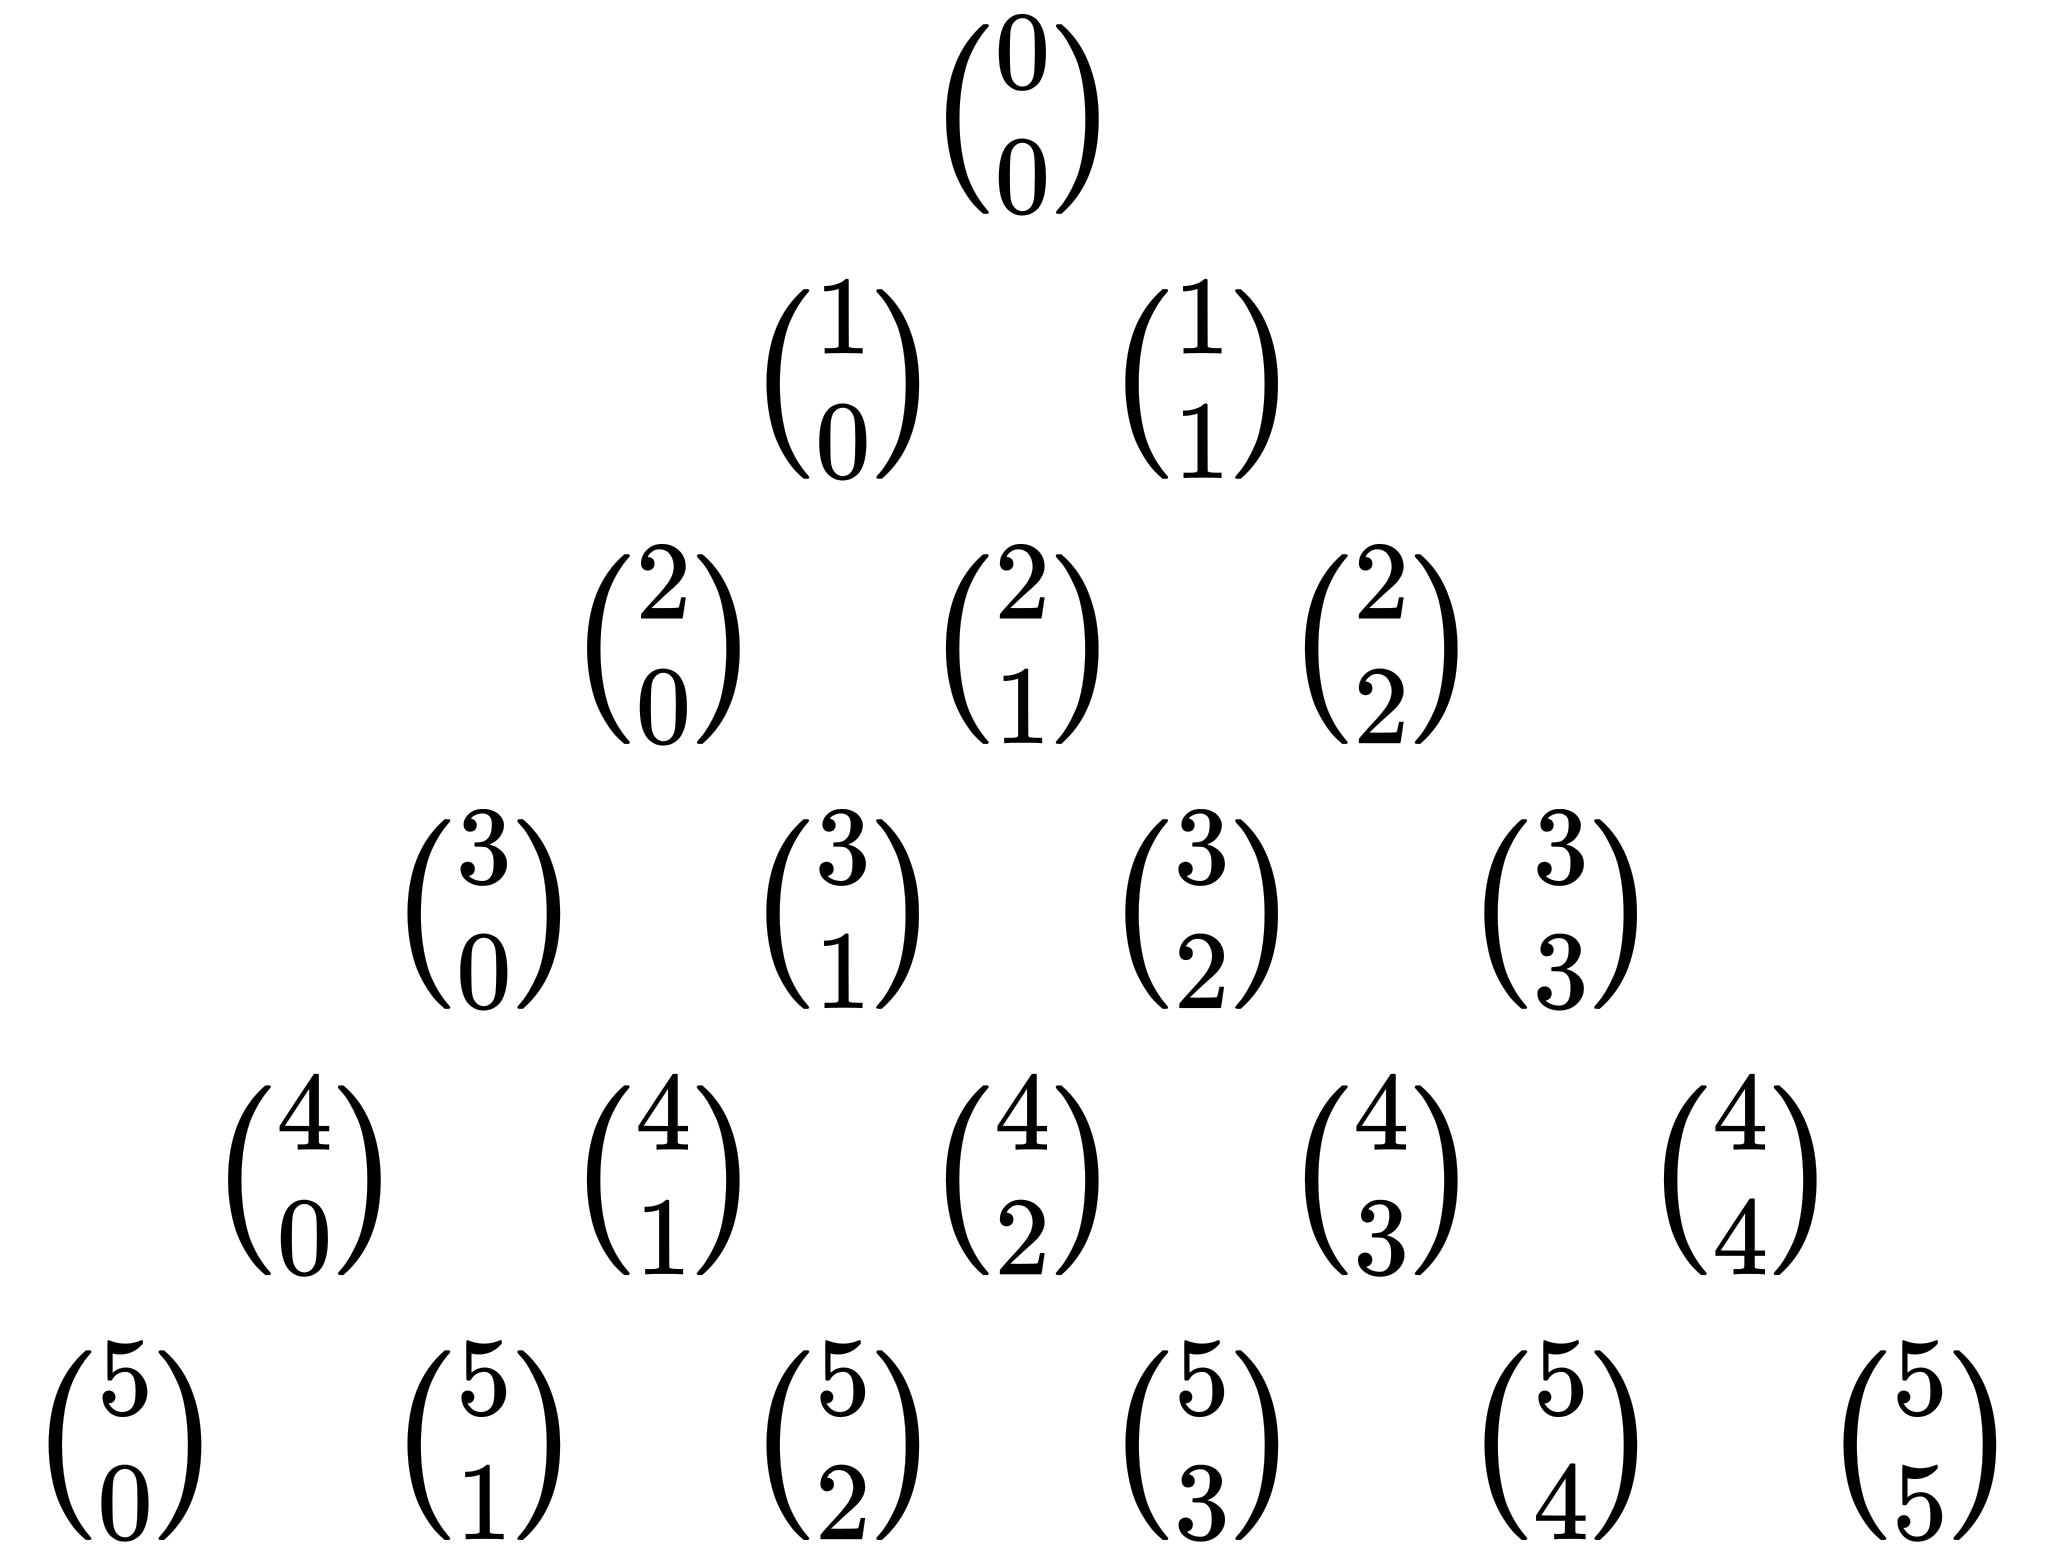
\includegraphics[width=0.25\textwidth]{pascals-binom}
    \caption{Pascal's Triangle - Binomial Coefficients}
\end{figure}
\begin{figure}[ht]
  \centering
    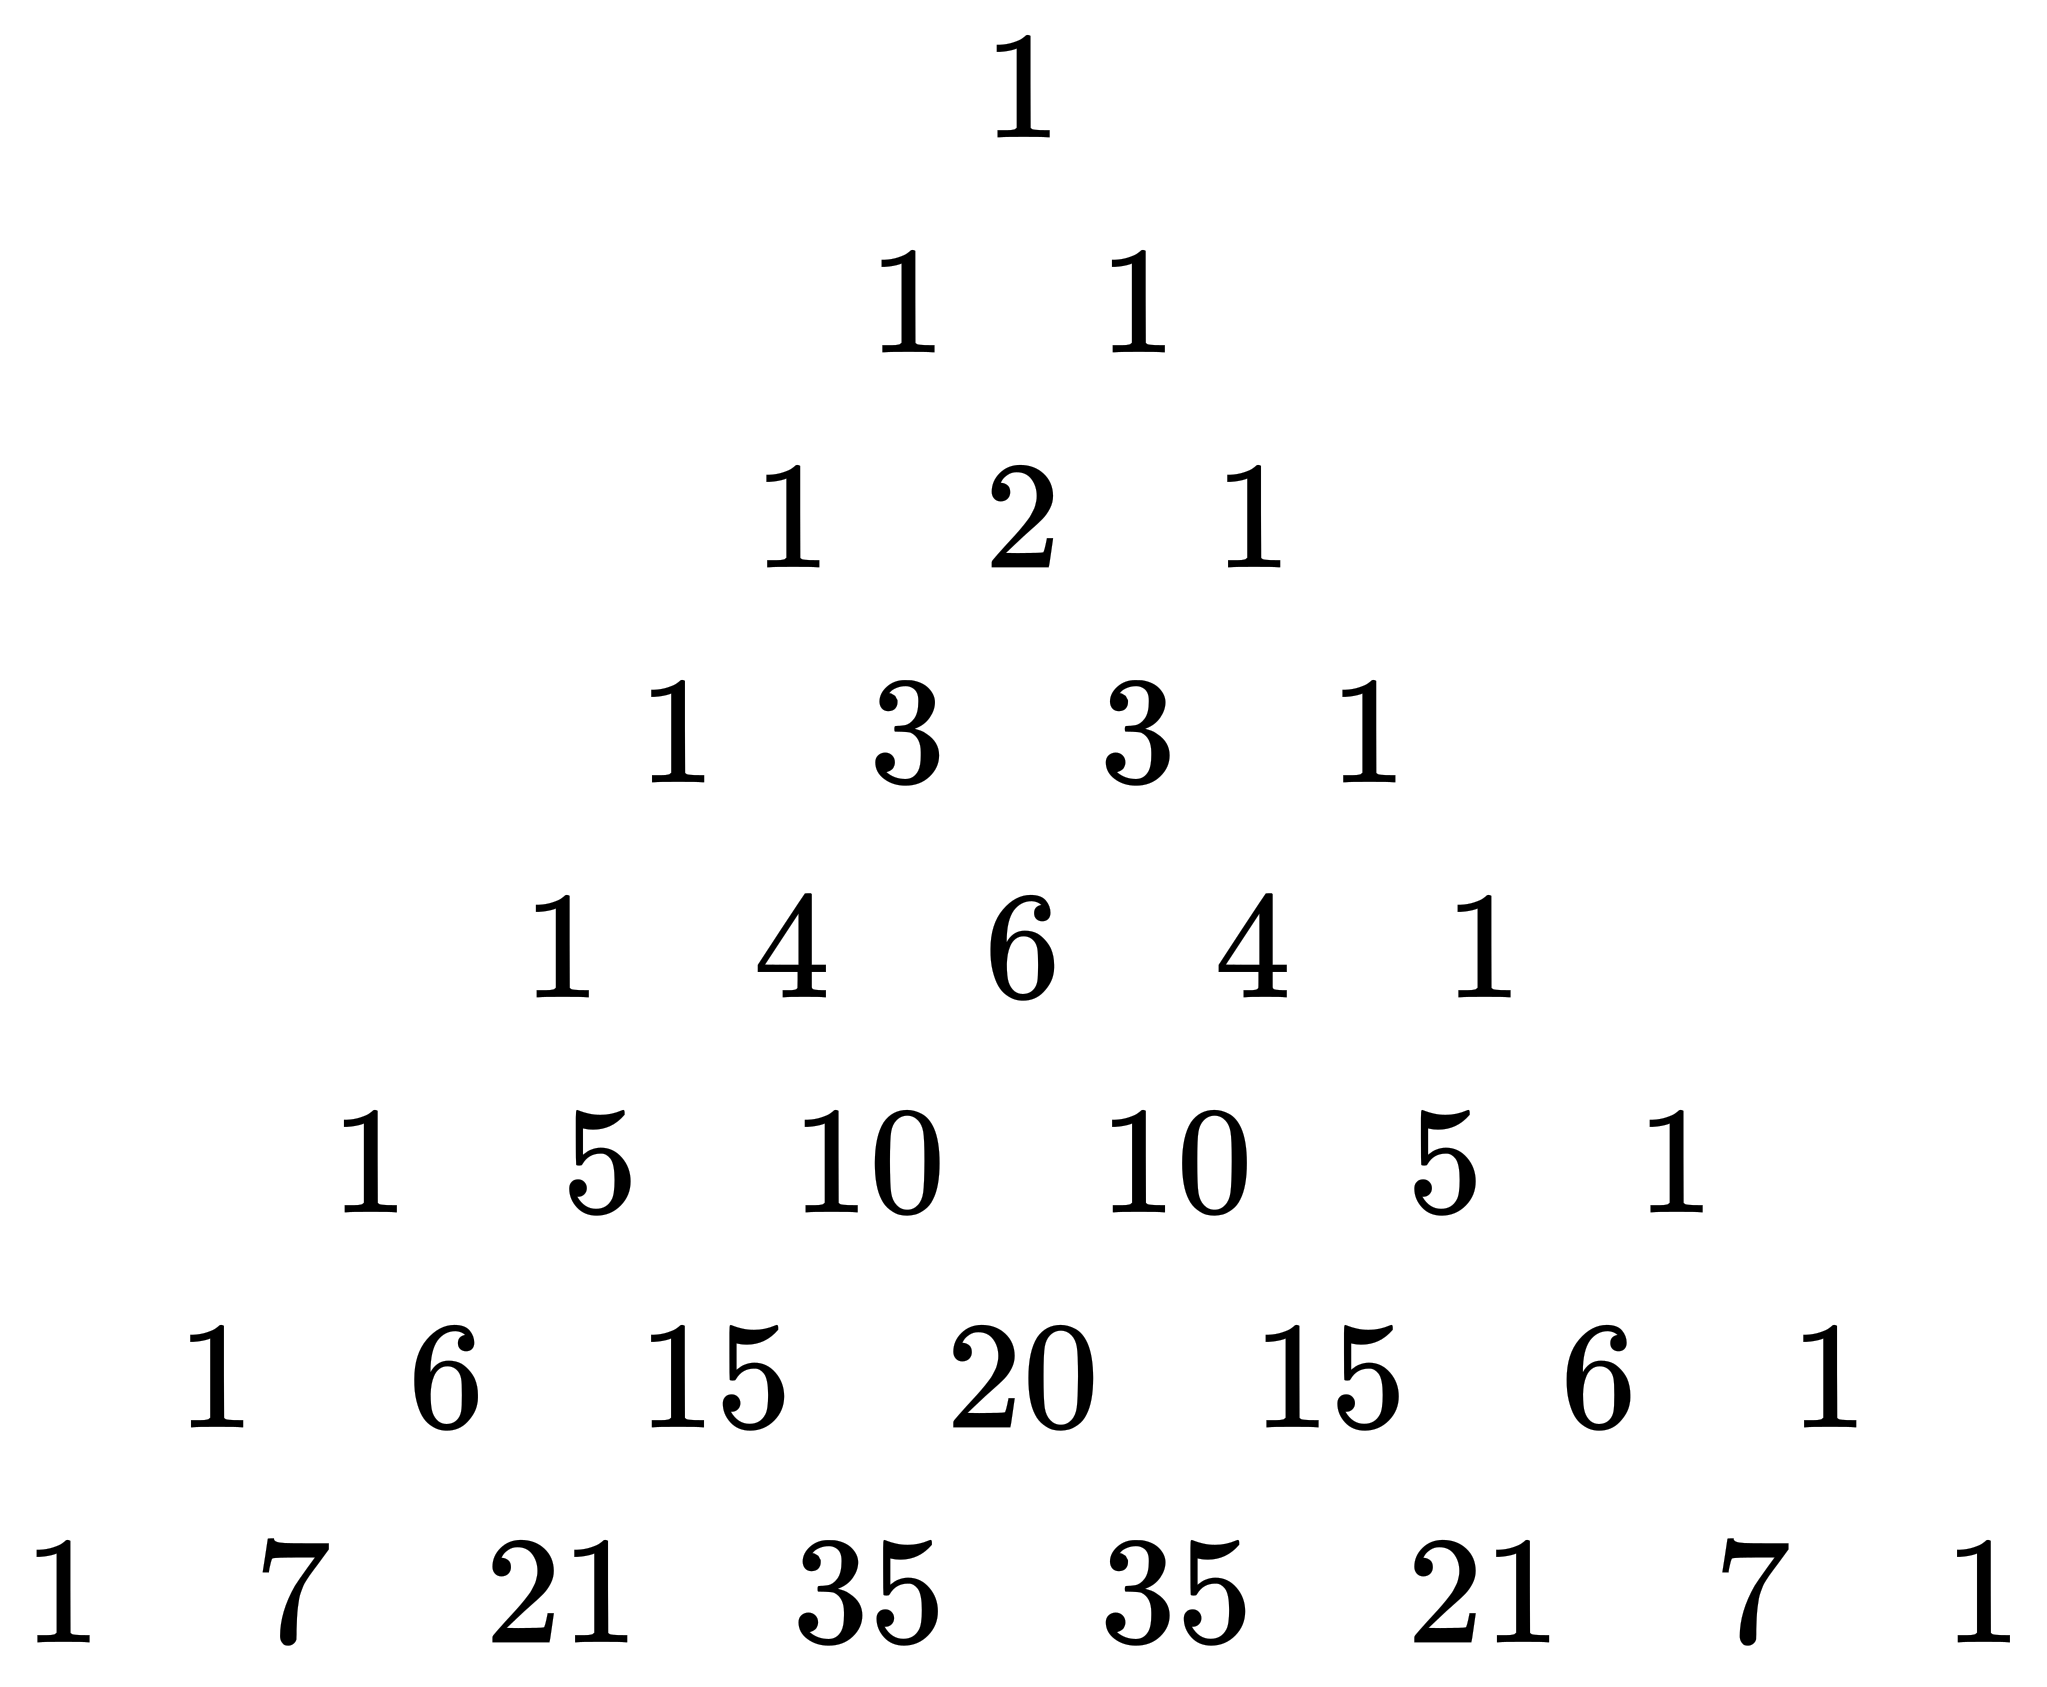
\includegraphics[width=0.25\textwidth]{pascals-trig}
    \caption{Pascal's Triangle - Numbers}
\end{figure}

\subsection{Characteristics}
\begin{itemize}
    \item We can see that each value is the sum of the two numbers above it.
    \item $\forall \; n \in \mathbb{N}: \binom{n}{0} = \binom{n}{n} = 1$
    \item $\forall \; n \in \mathbb{N}, 0 \leq k \leq n: \binom{n}{k} = \binom{n}{n-k}$
    \item \emph{Unimodality}:
$$
\begin{gathered}
 \binom{n}{k+1} \geq \binom{n}{k} \iff \frac{n!}{(k+1)!(n-k-1)!} \geq \frac{n!}{k!(n-k)!} \\
 \Updownarrow \\
 \frac{n-1}{2} \geq k
\end{gathered}
$$
In other words, the middle column of Pascal's Triangle always contains the
highest value in its row and the values decrease going left and going right.

 \item The sum of row $n$ is equal to $2^n$
$$
\begin{gathered}
    P([n]) \equiv \{A \mid A \subseteq [n]\} \\
    | 2^{[n]}| = |P([n])| = \;?
\end{gathered}
$$
\end{itemize}

\begin{claim}
$|P([n])|=2^n$

Given $S \subseteq A$:
$$\chi_s: A \to \{0,1\}$$
$$\chi_s(a) = \begin{cases}
    1 \quad a \in S \\
    0 \quad a \notin S
\end{cases}$$

We want to find a set $B$ such that $|B|=2^n$ so that there exists a function
$f: P([n]) \to B$ which is both \emph{injective} and \emph{surjective}.
\end{claim}

\begin{proof}
We define $B = \{f:[n] \to \{0,1\}\}$, and we know that $|B|=2^n$.

We define the function $T: P([n]) \to B$:
$$
\begin{gathered}
    \forall A \subseteq P([n]): A \in P([n]) \\
    T(A) = \chi_A = \begin{cases}
        1 \quad a \in A \\
        0 \quad a \notin A \\
    \end{cases}
\end{gathered}
$$

$T$ is \emph{one-to-one} and \emph{onto}:
$$f \in B \quad T^{-1}(f) = \{k \in [n] \mid f(k) = 1\}$$

\begin{conclusion}
$$|P([n])|=|B|=2^n$$
\end{conclusion}
\end{proof}
\section{Newton's Generalized Binomial Theorem}

$$
\begin{gathered}
(a+b)^n \\ \\
\begin{aligned}
    (a+b)^1 &= a+b \\
    (a+b)^2 &= \underbrace{\binom{2}{0}}_{1}b^2+ \underbrace{\binom{2}{1}}_{2}ab + \underbrace{\binom{2}{2}}_{1}a^2 \\
    (a+b)^3 &= \underbrace{\binom{3}{0}}_{1}b^3+ \underbrace{\binom{3}{1}}_{3}ab^2 + \underbrace{\binom{3}{2}}_{3}a^2b + \underbrace{\binom{3}{3}}_{1}a^3 \\
    (a+b)^n &= \sum_{k=0}^n \binom{n}{k} a^{k}b^{n-k}
\end{aligned} \\ \\
2^n = (1+1)^n= \sum_{k=0}^n \binom{n}{k}1^k1^{n-k} = \sum_{k=0}^{n} \binom{n}{k}
\end{gathered}
$$

Let's play which some more values for $a$ and $b$:
$$
\begin{gathered}
    (-1+1)^n=\sum_{k=0}^{n} \binom{n}{k}(-1)^k1^{n-k} =
    \sum_{k-0}^{n}\binom{n}{k}(-1)^k = 0 \\
    \Downarrow \\
    \binom{n}{0} - \binom{n}{1} + \binom{n}{2} - \binom{n}{3} + \dots +
    (-1)^k\binom{n}{n}=0 \\
    \Downarrow \\
    \binom{n}{0} + \binom{n}{2} + \binom{n}{4} + \dots = \binom{n}{1} + \binom{n}{3} +
    \binom{n}{5} + \dots
\end{gathered}
$$

\begin{conclusion}
In other words, the number of subsets of $[n]$ of even size is equal to the
number of subsets of $[n]$ of odd size.

We can show this easily if $n$ is odd by showing that $\binom{n}{k} = \binom{n}{n-k}$, which
allows us to draw a one-to-one symmetry from every term to its corresponding
equivalent term.
\end{conclusion}

\paragraph{Another proof}

Let there be $A\neq \emptyset$ of the size $n$ and $a \in A$.

$$
\begin{gathered}
    F_1=\{ B \subseteq A \mid |B| \text{ is even}\} \\
    F_2=\{ B \subseteq A \mid |B| \text{ is odd}\} \\
    \\
    f: F_1 \to F_1 \quad \forall B \in F_1: \\
    f(B)=\begin{cases}
        B \setminus \{a\} \quad a \in B \\
        B \cup \{a\} \quad a \notin B
    \end{cases}
\end{gathered}
$$
We see that if $|B|$ is even, then $|f(B)|$ is odd and $f(f(B))=B$. We also see
that $f$ is \emph{invertible} as it's \emph{one-to-one} and \emph{onto}, and therefore we see
that $|F_1|=|F_2|$.

\subsection{Generalizing the Binomial Theorem}

\begin{example}
$$
    (a+b+c)^{17}
$$
First, we know that for each term, the sum of powers of $a,b$ and $c$ will be
$17$. In regards to each term's coefficient, we can express it in the following
way:

"What is the coefficient of $a^3b^6c^8$?" is equivalent to asking how many ways
can we arrange in a row  3 $a$s, 6 $b$s and 8 $c$s, which can be expressed by
the following multinomial coefficient:
$$\binom{17}{3,6,8} = \frac{17!}{3!6!8!}$$
\end{example}


\subsection{Multinomial Theorem}

$$
\begin{gathered}
    m \in \mathbb{N} \quad (x_1+x_2+x_3+ \dots + x_n)^m \\
    = \sum_{\begin{subarray}{l}
        k_1,k_2,\dots,k_n \in \mathbb{N} \cup \{0\} \\
        k_1+k_2+\dots+k_n = m
    \end{subarray}}^n
    \binom{m}{k_1,k_2,\dots,k_n}
    x_1^{k_1}x_2^{k_2}x_3^{k_3}\dots x_n^{k_n}
\end{gathered}
$$

\section{Paths on a Grid}
\begin{example}
There are two delegates: $A$ and $B$, with $2k$ ballots ($k$ that have $A$ and
$k$ ballots have $B$). How many ways can we order the $2k$ ballots such that
there are never more ballots for $A$ than $B$? ($\# B \geq \# A$)

Similar problems include the ``line for the movies'' problem and ``number of
balanced series of $n$ parentheses'' (computer science).
$$\underbrace{()(())}_{\text{balanced}} \quad
\underbrace{())(()}_{\text{unbalanced}}$$

\end{example}
Algebraic expression:
$$A = \left\{a \in \{-1,1\}^{2n}\ \mid \sum_{i=1}^{2n} a_i = 0\right\} \quad |A|=\binom{2n}{n}$$
$$B=\left\{a \in A \mid \forall k \in [2n]: \sum_{i=1}^k a_i \leq 0\right\}
\quad |B|=\;?$$

\begin{figure}[ht]
  \centering
    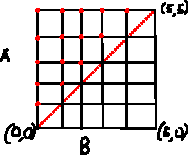
\includegraphics[width=0.25\textwidth]{w6-grid}
    \caption{Grid expression where $k=5$}
\end{figure}

\subsubsection{Symbols}
\begin{itemize}
    \item[A -] Total number of paths from $(0,0)$ to $(n,n)$ where $|A| = \binom{2n}{n}$
    \item[B -] Paths in A that do not go above the main diagonal
    \item[C -] Paths that go above the main diagonal
    $$
    \begin{gathered}
        B = A \setminus C \\
        |C| = |A| - |C| \Leftarrow C \subseteq A
    \end{gathered}
    $$
    \item[D -]Total number of paths from $(0,0)$ to $(n-1,n+1)$ where $|D|=\binom{2n}{n-1}$
\end{itemize}
\begin{claim}
How many ways are there to go from $(0,0)$ until $(n,n)$ without crossing the
main diagonal?

$$\frac{1}{n+1} \binom{2n}{n} = \binom{2n}{n} - \binom{2n}{n+1}$$
\end{claim}

$$|B| = |A| - |C| \underset{|C|=|D|}{=} |A| - |D| = \binom{2n}{n}-\binom{2n}{n+1}$$

We define $f: C \to D$:

Given $a \in C$, we symbolize $a=(a_1,a_2,\dots,a_n)$

$$A = \left\{a \in \{-1,1\}^n \mid \sum a_i = 0 \right\}$$
Where $-1$ is a step right and $1$ is a step up.

Where we need this to be true:
$$\sum_{i=1}^{k}a_i>0$$

$$k=\min\left\{1 \leq k\leq 2n \mid \sum_{i=1}^{k}a_i>0\right\}$$

$$(f(a))_i = \begin{cases}
    a_i & 1 \leq i \leq k \\
    -a_i & k < i
\end{cases}$$
We notice that for $f(a)$:
$$\sum_{i=1}^{2n}(f(a))_i = 2$$
Therefore we see that $f$ expresses the path between $(0,0)$ to $(n-1,n+1)$.
Notice that for  all $a \in C$:
$$f(f(a))=a \implies f \circ f |_C = \Id_C$$
\begin{proof}
$$
\begin{gathered}
    \implies f \text{ is \emph{invertible}} \\
    \implies |C| = |D| \\
    \implies |B| = C_n = \binom{2n}{n} - \binom{2n}{n+1}
\end{gathered}
$$
\end{proof}

\end{document}
